\begin{singlespace}
    \chapter{\textbf{The relative cost of resource use for photosynthesis drives variance in leaf nitrogen content across climate and soil resource availability gradients}}
\end{singlespace}

\section{Introduction}
Terrestrial biosphere models, which comprise the land surface component of Earth system models, are sensitive to the formulation of photosynthetic processes \shortcite{Knorr2000,Ziehn2011,Booth2012}. This is because photosynthesis is the largest carbon flux between the atmosphere and terrestrial biosphere, and is constrained by ecosystem carbon and nutrient cycles \shortcite{Hungate2003,LeBauer2008,IPCC2021,Fay2015}. Many terrestrial biosphere models formulate photosynthesis by parameterizing photosynthetic capacity within plant functional groups through empirical linear relationships between area-based leaf nitrogen content ($N_\mathrm{area}$) and the maximum carboxylation rate of Ribulose-1,5-bisphosphate carboxylase/oxygenase \shortcite{Kattge2009,Rogers2014,Rogers2017a}. Models are also beginning to include connected carbon-nitrogen cycles \shortcite{Wieder2015_NPP,Shi2016,Davies-Barnard2020,Braghiere2022}, which allows leaf photosynthesis to be predicted directly through changes in $N_{\mathrm{area}}$ and indirectly through changes in soil nitrogen availability (e.g., LPJ-GUESS, Smith et al., 2014; CLM5.0, Lawrence et al., 2019). Despite recent model developments, open questions remain regarding the generality of ecological relationships between soil nitrogen availability, leaf nitrogen content, and leaf photosynthesis across edaphic and climatic gradients.

Empirical support for positive relationships between soil nitrogen availability and $N_\mathrm{area}$ is abundant \shortcite{Firn2019,Liang2020}, and is a result often attributed to the high nitrogen cost of building and maintaining Rubisco \shortcite{Evans1989_photoN,EvansSeemann1989,Onoda2004,Onoda2017,Dong2020}. Such patterns imply that positive relationships between soil nitrogen availability and $N_\mathrm{area}$ should cause an increase in leaf photosynthesis and photosynthetic capacity by increasing the maximum rate of Rubisco carboxylation through increased investments to Rubisco construction and maintenance. This integrated $N_\mathrm{area}$-photosynthesis response to soil nitrogen availability has been observed both in manipulative experiments and across environmental gradients \shortcite{Field1986,Evans1989_photoN,Walker2014,Li2020}, and is thought to be driven by ecosystem nitrogen limitation, which limits primary productivity globally \shortcite{LeBauer2008,Fay2015}. However, this response is not consistently observed, as recent studies note variable $N_\mathrm{area}$-photosynthesis relationships across soil nitrogen availability gradients \shortcite{Liang2020,Luo2021} and that aboveground growing conditions (e.g., light availability, temperature, vapor pressure deficit) or species identity traits (e.g., photosynthetic pathway, nitrogen acquisition strategy) may be more important for explaining variance in $N_\mathrm{area}$ and photosynthetic capacity across time and space \shortcite{Adams2016,Dong2017,Dong2020,Dong2022a,Smith2019,Peng2021,Westerband2023}.

\section{Methods}

\subsection{textit{Site descriptions and sampling methodology}}

We collected leaf and soil samples from 24 open grassland sites across central and eastern Texas in summer 2020 and summer 2021 (Fig. \ref{fig:figure4.1}). Twelve sites were visited between June and July 2020 and 14 sites (11 unique from 2020) were visited between May and June 2021 (Table 1). We explicitly chose sites that maximized variability in precipitation and edaphic variability between sites while minimizing temperature variability across the environmental gradient (Table 1). No site with personally communicated or anecdotal evidence of grazing or disturbance (e.g., mowing, feral hog activity, etc.) were used. We collected leaf material from three individuals each of the five most abundant species at random locations at each site, only  selecting species that were broadly classified as graminoid, forb/herb, shrub, or subshrub growth habits per the USDA PLANTS database \shortcite{USDANRCS2022}. All collected leaves were fully expanded with no visible herbivory or other external damage and also free from shading by nearby shrubs or trees. Five soil samples were collected from 0-15cm below the soil surface at each site near the leaf collection sample locations. Soil samples were later mixed together by hand to create one composite soil sample per site.

\subsection{\textit{Leaf trait measurements}}
Images of each leaf were taken immediately following each site visit using a flat-bed scanner. Fresh leaf area was determined from each image using the 'LeafArea' R package \shortcite{Katabuchi2015}, which automates leaf area calculations using ImageJ software \shortcite{Schneider2012}. Each leaf was dried at 65\textdegree{}C for at least 48 hours to a constant mass, weighed, and manually ground in a mortar and pestle until homogenized. Leaf mass per area ($M_\mathrm{area}$; $\mathrm{g\ m^{-2}}$) was calculated as the ratio of dry leaf biomass to fresh leaf area. Subsamples of dried and homogenized leaf tissue were used to measure leaf nitrogen content ($N_\mathrm{mass}$; $\mathrm{gN\ g^{-1}}$) through elemental combustion analysis (Costech-4010, Costech Instruments, Valencia, CA). Leaf nitrogen content per unit leaf area ($N_area$; $\mathrm{gN\ m^{-2}}$) was then calculated as the product of $N_\mathrm{mass}$ and $M_\mathrm{area}$.
    
Subsamples of dried and homogenized leaf tissue were sent to the University of California-Davis Stable Isotope Facility to determine leaf $\delta^{13}$C. Leaf $\delta^{13}$C values were determined using an elemental analyzer (PDZ Europa ANCA-GSL; Sercon Ltd., Chestshire, UK) interfaced to an isotope ratio mass spectrometer (PDZ Europa 20-20 Isotope Ratio Mass Spectrometer, Sercon Ltd., Chestshire, UK). We used leaf $\delta^{13}$C values (‰; relative to Vienna Pee Dee Belemnite international reference standard) to estimate the ratio of intercellular ($C_\mathrm{i}$) to extracellular ($C_\mathrm{a}$) CO\textsubscript{2} ratio (leaf $C_\mathrm{i}$:$C_\mathrm{a}$, $\chi$; unitless) following the approach of Farquhar et al. (1989) described in Cernusak et al. (2013). We derived $\chi$ as:

\begin{equation} 
    \label{eq_4.1}
    \chi=\frac{C_{i}}{C_{a}}=\frac{\Delta^{13}C - a}{b - a}
\end{equation}
    
\noindent where $\Delta^{13}$C represents the relative difference between leaf $\delta^{13}$C (‰) and air $\delta^{13}$C (‰), and is calculated as:

\begin{equation}
    \label{eq_4.2}
    \Delta^{13}C = \frac{\delta^{13}C_{air} - \delta^{13}C_{leaf}}{1 + \delta^{13}C_{leaf}}
\end{equation}

\noindent $\delta^{13}\mathrm{C_{air}}$, traditionally assumed to be -8‰ \shortcite{Keeling1979,Farquhar1989}, was calculated as a function of calendar year \textit{t} using an empirical equation derived in \shortciteN{Feng1999}:

\begin{equation}
    \label{eq_4.3}
    \delta^{13}C_{air} = -6.429 - 0.006e^{0.0217(t-1740)}
\end{equation}
    
 \noindent This calculation resulted in $\delta^{13}\mathrm{C_{air}}$ values for 2020 and 2021 as -9.04 and -9.09, respectively. a represents the fractionation between $^{12}\mathrm{C}$ and $^{13}\mathrm{C}$ due to diffusion in air, assumed to be 4.4‰, and b represents the fractionation caused by Rubisco carboxylation, assumed to be 27‰ \shortcite{Farquhar1989}. For $C_{4}$ species, b in Eqn. \ref{eq_4.1} was set to 6.3‰, and was derived from:

\begin{equation}
    \label{eq_4.4}
    b = c + (d \cdot \phi)
\end{equation}
    
\noindent Where c was set to -5.7‰ and d was set to 30‰ \shortcite{Farquhar1989}. $\phi$, which is the bundle sheath leakiness term, was set to 0.4. All $\chi$ values less than 0.2 and greater than 1.0 were assumed to be incorrect and removed.
    
We derived the unit cost of resource use ($\beta$) using leaf $\chi$ and site climate data with equations first described in \shortciteN{Prentice2014} and simplified in \shortciteN{Lavergne2020}:

\begin{equation}
    \label{eq_4.5}
    \beta = 1.6\eta^{*} D \frac{\chi - (\frac{\Gamma^*}{C_{a}})^{2}}{(1 - \chi)^{2}(K_{m} + \Gamma^{*})}
\end{equation}
    
\noindent where $\eta^{*}$ is the viscosity of water relative to 25\textdegree{}C, calculated using elevation and mean air temperature of the seven days leading up to each site visit following equations in \shortciteN{Huber2009}. D represents vapor pressure deficit (Pa), set to the mean vapor pressure deficit of the seven days leading up to each site visit, $C_\mathrm{a}$ represents atmospheric CO\textsubscript{2} concentration, arbitrarily set to 420 $\mathrm{\mu mol\ mol^{-1}}$ CO\textsuperscript{2}. $K_\mathrm{m}$ (Pa) is the Michaelis-Menten coefficient for Rubisco affinity to CO\textsubscript{2} and O\textsubscript{2}, calculated as:
    
\begin{equation} \label{eq_4.6}
    K_{m} = K_{c} \cdot \left ( 1 + \frac{O_i}{K_o} \right )
\end{equation}

\noindent where $K_\mathrm{c}$ (Pa) and $K_\mathrm{o}$ (Pa) are the Michaelis-Menten coefficients for Rubisco affinity to CO\textsubscript{2} and O\textsubscript{2}, respectively, and $O_\mathrm{i}$  is the intercellular O\textsubscript{2} concentration. $\Gamma^{*}$ (Pa) is the CO\textsubscript{2} compensation point in the absence of dark respiration. $K_\mathrm{c}$, $K_\mathrm{o}$, and $\Gamma^{*}$ were determined using equations described in \shortciteN{Medlyn2002} and derived in \shortciteN{Bernacchi2001}, invoking an elevation correction for atmospheric pressure as explained in \shortciteN{Stocker2020}.
\clearpage

\newpage
placeholder for Table 1
\clearpage

\newpage
\begin{landscape}
    \begin{figure}
        \centering
        \includegraphics[scale = 0.05]{ch4_TXeco/figs/TXeco_fig1_site_map.png}
        \caption[Maps that detail site locations along 2006-2020 mean annual precipitation (panel A) and mean annual temperature (panel B) gradients in Texas, USA.]{Maps that detail site locations along 2006-2020 mean annual precipitation (panel A) and mean annual temperature (panel B) gradients in Texas, USA. Precipitation and temperature data were plotted at a 4-km grid resolution and are masked to include only grid cells that occur in the Texas state boundary in the United States. In both panels, open circles refer to sites visited in 2020, open triangles to sites visited in 2021, and closed circles to sites visited in 2020 and 2021. The scale bar in panel A also applies to panel B.}
        \label{fig:figure4.1}
    \end{figure}
\end{landscape}
\clearpage

\subsection{\textit{Site climate data}}
We used the Parameter-elevation Regressions on Independent Slopes Model (PRISM) \shortcite{Daly2008}climate product to access gridded daily temperature and precipitation data for the coterminous United States at a 4-km grid resolution between January 1, 2006 and July 31, 2021 (PRISM Climate Group, Oregon State University, https://prism.oregonstate.edu, data created 4 Feb 2014, accessed 24 Mar 2022). Daily mean air temperature, mean VPD, and total precipitation data were extracted from the grid cell that contained the latitude and longitude of each property using the ‘extract’ function in the ‘terra’ R package \shortcite{Hijmans2022}. PRISM data were used in lieu of local weather station data because several rural sites did not have a local weather station present within a 20-km radius of the site. Daily site climate data were used to estimate mean annual precipitation and mean annual temperature for each site between 2006 and 2020 (Table 1). We then calculated total precipitation and mean daily VPD for the prior 1, 2, 3, 4, 5, 6, 7, 8, 9, 10, 15, 20, 25, 30, 60, and 90 days leading up to each site visit.

\subsection{\textit{Site edaphic characteristics}}
Subsamples of composited soil samples were sent to the Texas A \& M Soil, Water and Forage Laboratory to quantify soil nitrate concentration (NO3-N; ppm). Soil NO$_{3}$-N was determined by extracting composite soil samples in 1 M KCl, measuring absorbance values of extracts at 520 nm using the end product of a NO$_{3}$-N to NO$_{2}$-N cadmium reduction reaction \shortcite{Kachurina2000}. Soil texture data from 0-15cm below the soil surface were accessed using the SoilGrids2.0 data product \shortcite{Poggio2021} through the ‘fetchSoilGrids’ function in the ‘soilDB’ R package \shortcite{Beaudette2022}. We used SoilGrids2.0 to access soil texture data in lieu of analyses using the collected composite soil sample due to a lack of soil material from some sites after sending samples for soil NO$_{3}$-N.

Soil moisture was not measured in the field, but was estimated using the ‘Simple Process-Led Algorithms for Simulating Habitats’ model ('SPLASH') \shortcite{Davis2017}. This model, derived from the STASH model \shortcite{Cramer1988}, spins up a bucket model using Priestley-Taylor equations \shortcite{Priestley1972} to calculate daily soil moisture (Wn; mm) as a function of the previous day’s soil moisture ($W_\mathrm{n}{}^{-1}$; mm), daily precipitation ($P_\mathrm{n}$; mm), condensation ($C_\mathrm{n}$; mm), actual evapotranspiration ($E_{n}^a$; mm), and runoff (RO; mm):

\begin{equation}
    \label{eq_4.7}
    W_n = W_{n-1} + P_n + C_n - E_{n}^{a} - RO
\end{equation}

Models were spun up by equilibrating the previous day’s soil moisture using successive model iterations with daily mean air temperature, daily precipitation total, the number of daily sunlight hours, and latitude as model inputs \shortcite{Davis2017}. Daily sunlight hours were estimated for each day at each site using the ‘getSunlightTimes’ function in the ‘suncalc’ R package, which estimated sunrise and sunset times of each property using date and site coordinates \shortcite{Thieurmel2019}. Water holding capacity (mm), or bucket size, was estimated as a function of soil texture using pedotransfer equations explained in \shortciteN{Saxton2006}, as done in \shortciteN{Stocker2020} and \shortciteN{Bloomfield2022}. A summary of these equations is included in the Supplemental Information.

Daily soil moisture outputs from the SPLASH model for each site were used to calculate mean daily soil moisture for the prior 1, 2, 3, 4, 5, 6, 7, 8, 9, 10, 15, 20, 25, 30, 60, and 90 days leading up to each site visit. Mean daily soil moisture values were then expressed as a fraction of water holding capacity to normalize across sites with different bucket depths, as done in \shortciteN{Stocker2018}.

\subsection{\textit{Plant functional group assignments}}
Plant functional group was assigned to each species and used as the primary descriptor of species identity. Specifically, we assigned plant functional groups based on photosynthetic pathway (C$_3$, C$_4$) and ability to form associations with symbiotic nitrogen-fixing bacteria. The ability to form associations with symbiotic nitrogen-fixing bacteria was assigned based on whether species were in the \textit{Fabaceae} family, and photosynthetic pathway of each species was determined from past literature and confirmed through leaf $\delta^{13}$C values. We chose these plant functional groups based on \textit{a priori} hypotheses regarding the functional role of nitrogen fixation and photosynthetic pathway on the sensitivity of plant nitrogen uptake and leaf nitrogen allocation to soil nutrient availability and aboveground growing conditions. These plant functional group classifications resulted in three distinct plant functional groups within our dataset: C$_3$ legumes (n = 53), C$_3$ non-legumes (n = 350), and C$_4$ non-legumes (n = 117).

\subsection{\textit{Data analysis}}
All analyses and plotting were conducted in R version 4.1.1 \shortcite{RCoreTeam2021}. We constructed a series of separate linear mixed-effects models to investigate environmental drivers of $\beta$, $\chi$, $N_\mathrm{area}$, $N_\mathrm{mass}$, and $M_\mathrm{area}$, followed by a path analysis using a piecewise structural equation model to investigate direct and indirect effects of climate and soil resource availability on $N_\mathrm{area}$.

To explore environmental drivers of $\beta$, we built a linear mixed-effects model that included soil moisture, soil nitrogen availability, and plant functional group as fixed effect coefficients. Species were designated as a random intercept term. Interaction coefficients between all possible combinations of the three fixed effect coefficients were also included. $\beta$ was natural log transformed to linearize data. We used an information-theoretic model selection approach to determine whether 90-, 60-, 30-, 20-, 15-, 10-, 9-, 8-, 7-, 6-, 5-, 4-, 3-, 2-, or 1-day mean daily soil moisture conferred the best model fit for $\beta$. To do this, we constructed 16 separate linear mixed-effects models where log-transformed $\beta$ was included as the response variable and each soil moisture timestep was separately included as a single continuous fixed effect. Species were included as a random intercept term for all models. We used corrected Akaike Information Criterion (AICc) to select the soil moisture timescale that conferred the best model fit, indicated by the model with the lowest AICc score (Table S2; Fig. S2).

To explore environmental drivers of $\chi$, we constructed a second linear mixed effects model that included VPD, soil moisture, soil nitrogen availability, and plant functional group as fixed effect coefficients. Two-way interactions between plant functional group and VPD, soil nitrogen availability, or soil moisture were also included as fixed effect coefficients, in addition to a three-way interaction between soil moisture, soil nitrogen availability, and plant functional group. Species were included as a random intercept term. We used an information-theoretic model selection approach to determine whether 90-, 60-, 30-, 20-, 15-, 10-, 9-, 8-, 7-, 6-, 5-, 4-, 3-, 2-, or 1-day mean daily VPD conferred the best model fit for $\chi$ using the same approach explained above for the soil moisture effect on $\beta$. The soil moisture timescale was set to the same timescale that conferred the best fit for $\beta$.

To explore environmental drivers of $N_\mathrm{area}$, $N_\mathrm{mass}$, and $M_\mathrm{area}$, we constructed three separate linear mixed effects model that each included $\chi$, soil nitrogen availability, soil moisture, and plant functional group as fixed effect coefficients. Two-way interactions between plant functional group and $\beta$, $\chi$, soil nitrogen availability, or soil moisture were included as additional fixed effect coefficients, in addition to a three-way interaction between soil nitrogen availability, soil moisture, and plant functional group. Species were included as a random intercept term, with the soil moisture timescale set to the same timescale that conferred the best fit for $\beta$.

In all linear mixed-effects models explained above, including those to select relevant timescales, we used the 'lmer' function in the 'lme4' R package \shortcite{Bates2015} to fit each model and the 'Anova' function in the 'car' R package \shortcite{Fox2019} to calculate Type II Wald's $\chi^2$ and determine the significance level ($\alpha$ = 0.05) of each fixed effect coefficient. We also used the 'emmeans' R package \shortcite{Lenth2019} to conduct post-hoc comparisons using Tukey's tests, where degrees of freedom were approximated using the Kenward-Roger approach \shortcite{Kenward1997}. Trendlines and error ribbons for all plots were drawn using a series of ‘emmeans’ outputs across the range in plotted x-axis values.

Finally, we conducted a path analysis using a piecewise structural equation model to examine direct and indirect pathways that determined variance in $N_\mathrm{area}$. Seven separate linear mixed effects models were loaded into the piecewise structural equation model. Models were constructed per our \textit{a priori} hypotheses following patterns expected from photosynthetic least-cost theory. The first model regressed $N_\mathrm{area}$ against $\chi$, $N_\mathrm{mass}$, and $M_\mathrm{area}$. The second model regressed Marea against $\chi$. The third model regressed $N_\mathrm{mass}$ against $\chi$ and $M_\mathrm{area}$ \shortcite{Dong2017,Dong2020}. The fourth model regressed $\chi$ against $\beta$ and VPD. The fifth model regressed $\beta$ against soil nitrogen availability, soil moisture, ability to associate with symbiotic nitrogen-fixing bacteria, and photosynthetic pathway. The sixth model regressed soil nitrogen availability against soil moisture, while the seventh model regressed VPD against soil moisture \shortcite{Novick2016,Sulman2016}. All models included the relevant timescale selected in the individual linear mixed effect models explained above (2-day soil moisture, 4-day vapor pressure deficit). Models also included species as a random intercept term, were built using the ‘lme’ function in the ‘nlme’ R package \shortcite{Pinheiro2022}, and subsequently loaded into the piecewise structural equation model using the ‘psem’ function in the ‘piecewiseSEM’ R package \shortcite{Lefcheck2016}.

\section{Results}
\subsection{\textit{Cost to acquire nitrogen relative to water ($\beta$)}}
Model selection indicated that 2-day soil moisture was the timescale that conferred the best model fit for $\beta$ (AICc = 1227.83; Table S2; Fig. S1). Increasing soil nitrogen availability generally decreased $\beta$ (\textit{p} < 0.001; Table 2), a pattern driven by a negative effect of increasing soil nitrogen availability on $\beta$ in C$_3$ nonlegumes (Tukey: \textit{p} < 0.001) and C$_3$ legumes (Tukey: \textit{p} = 0.004; Fig. 2a). C$_4$ nonlegumes also demonstrated a negative trend in the effect of increasing soil nitrogen availability on $\beta$, but this pattern was not significantly different from zero (Tukey: \textit{p} = 0.307; Fig. 2a). There was no apparent effect of soil moisture on $\beta$ (\textit{p} = 0.264; Table 1; Fig. 2b). A functional group effect (\textit{p} < 0.001; Table 1) indicated that C$_4$ nonlegumes generally had lower $\beta$ values than both C$_3$ legumes and C$_3$ non-legumes when averaged across soil moisture and soil nitrogen availability values (Tukey: p < 0.001 in both cases), while average $\beta$ values in C$_3$ legumes did not differ from C$_3$ nonlegumes (Tukey: \textit{p} = 0.691).

\newpage
placeholder Table 2
\clearpage

\newpage
\begin{landscape}
    \begin{figure}
    \centering
    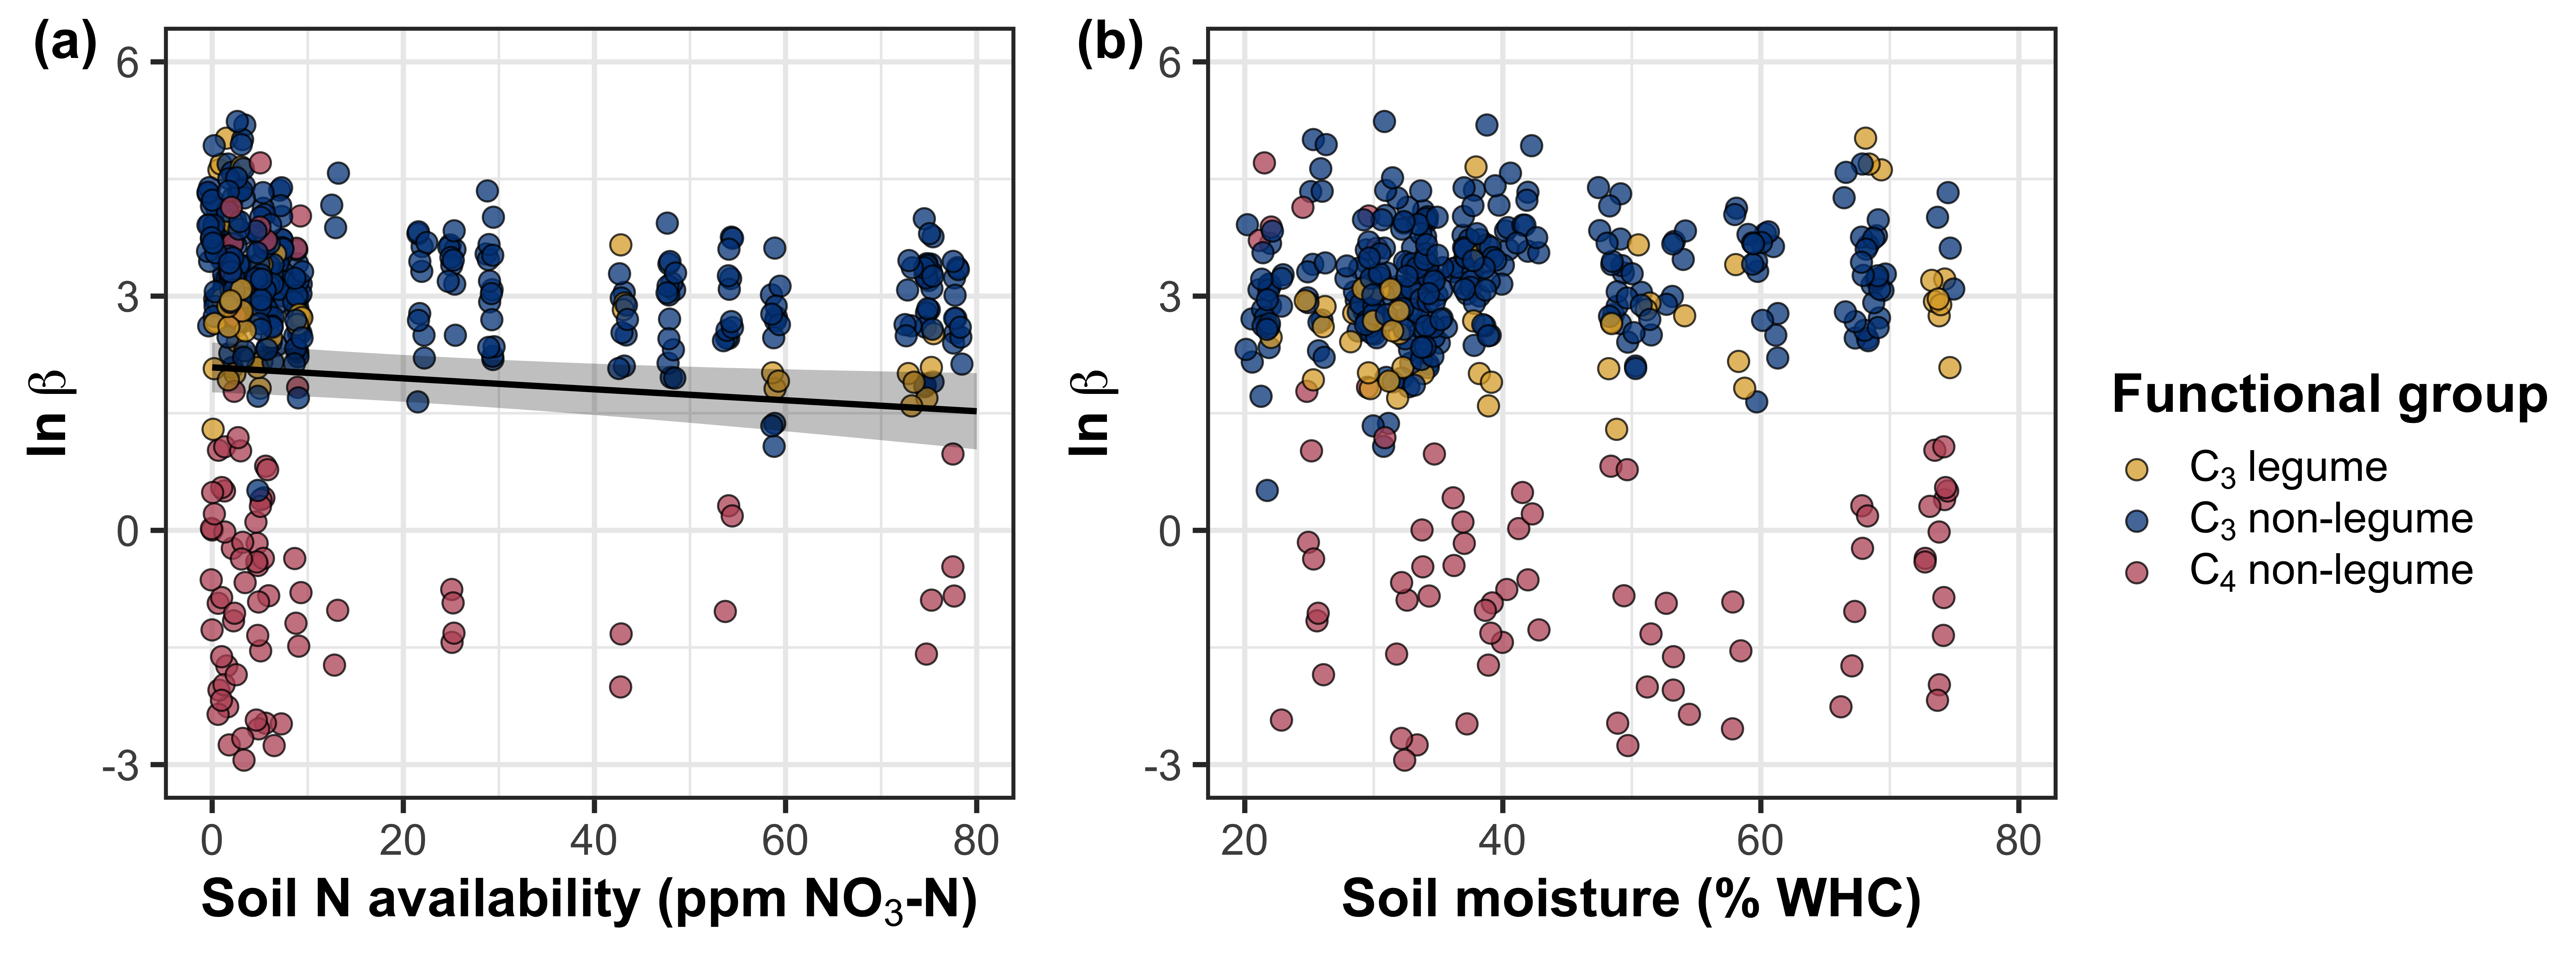
\includegraphics[scale = 0.075]{ch4_TXeco/figs/TXeco_fig2_beta.png}
    \caption[Effects of soil nitrogen availability and soil moisture on the unit cost ratio $\beta$]{Effects of soil nitrogen availability (a) and soil moisture (b) on the unit cost ratio $\beta$. In (b), soil moisture is represented as a percent of site water holding capacity. Yellow shading and trendlines indicate C$_3$ legumes, blue shading and trendlines indicate C$_3$ non-legumes, and red shading and trendlines indicate C$_4$ non-legumes. Points are jittered for visibility. Variably colored trendlines are only included if there is an interaction between the x-axis and plant functional group, where solid trendlines indicate slopes that are different from zero (\textit{p} < 0.05) and dashed trendlines indicate slopes that are not different from zero (\textit{p} < 0.05). Error ribbons represent the upper and lower 95\% confidence intervals of each fitted trendline.}
    \label{fig:figure4.2}
\end{figure}
\end{landscape}
\clearpage

\subsection{\textit{Leaf C\textsubscript{i}:C\textsubscript{a}}}
Model selection indicated that 4-day daily VPD was the timescale that conferred the best model fit for $\chi$ (AICc = -883.97; Table S1; Fig. S2).

Variance in $\chi$ was driven by a series of two-way interactions between functional group and VPD (\textit{p} = 0.006; Table 3), soil moisture (\textit{p} = 0.033, Table 3), and soil nitrogen availability (\textit{p} = 0.022; Table 3). The interaction between 4-day VPD and functional group revealed that the general negative effect of increasing VPD (\textit{p} < 0.001; Table 3) was driven by a negative effect of increasing VPD on $\chi$ in C$_3$ nonlegumes (Tukey: \textit{p} < 0.001) and marginal negative effect in C$_3$ legumes (Tukey: \textit{p} = 0.074) paired with a positive trending, but insignificant effect of increasing VPD in C$_4$ nonlegumes (Tukey: \textit{p} = 0.130; Fig. 3a). The interaction between 2-day soil moisture and functional group indicated that the general negative effect of increasing soil moisture on $\chi$ was driven by a positive effect of increasing soil moisture on $\chi$ in C$_4$ nonlegumes (Tukey: \textit{p} = 0.009) despite a positive trending but insignificant effect of increasing soil moisture on $\chi$ in C$_3$ legumes (Tukey: \textit{p} = 0.116) and a null effect of soil moisture on $\chi$ in C$_3$ nonlegumes (Tukey: \textit{p} = 0.693; Fig. 3c). The interaction between soil nitrogen availability and plant functional group revealed a weak negative effect of increasing soil nitrogen availability on $\chi$ in C$_3$ legumes (Tukey: \textit{p} = 0.045), with no apparent effect in C$_3$ nonlegumes (Tukey: \textit{p} = 0.706) or C$_4$ nonlegumes (Tukey: \textit{p} = 0.757). Finally, an individual effect of functional group (\textit{p} < 0.001; Table 3) revealed that C$_4$ nonlegumes generally had lower $\chi$ than C$_3$ legumes and C$_3$ nonlegumes (Tukey: \textit{p} < 0.001 in both cases), with no apparent difference between C$_3$ legumes and C$_3$ nonlegumes (Tukey: \textit{p} = 0.831).

\newpage
placeholder Table 3
\clearpage

\newpage
\begin{figure}
    \centering
    
\includegraphics[scale = 0.2]{ch4_TXeco/figs/TXeco_fig3_chi.png}
    \caption[Effects of 4-day mean vapor pressure deficit, 2-day soil moisture (per water holding capacity), and soil nitrogen availability on $\chi$. ]{Effects of 4-day mean vapor pressure deficit (a), 2-day soil moisture (per water holding capacity; b), and soil nitrogen availability (c) on $\chi$. Shading and trendlines are as explained in Figure 2. Points are jittered for visibility. Variably colored trendlines are only included if there is an interaction between the x-axis and plant functional group, where solid trendlines indicate slopes that are different from zero (\textit{p} < 0.05) and dashed trendlines indicate slopes that are not different from zero (\textit{p} < 0.05). Error ribbons represent the upper and lower 95\% confidence intervals of each fitted trendline.}
    \label{fig:figure4.3}
\end{figure}
\clearpage

\subsection{\textit{Leaf nitrogen content}}
An interaction between $\chi$ and plant functional group (\textit{p} < 0.001; Table 4) revealed that the general negative effect of increasing $\chi$ on $N_\mathrm{area}$ (\textit{p} < 0.001; Table 4) was driven by a negative effect of increasing $\chi$ on $N_\mathrm{area}$ in C$_3$ nonlegumes (Tukey: \textit{p} < 0.001) and C$_3$ legumes (Tukey: \textit{p} = 0.002) despite a null effect of $\chi$ on $N_\mathrm{area}$ in C$_4$ nonlegumes (Tukey: \textit{p} = 0.795; Fig. 4a). An interaction between soil nitrogen availability and soil moisture (\textit{p} = 0.028; Table 4) indicated that the marginal positive effect of increasing soil nitrogen availability on $N_\mathrm{area}$ (\textit{p} = 0.091; Table 4) decreased with increasing soil moisture, despite no apparent individual effect of soil moisture on $N_\mathrm{area}$ (\textit{p} = 0.692; Table 4). Finally, a plant functional group effect (\textit{p} < 0.001; Table 4) indicated that C$_4$ nonlegumes had lower $N_\mathrm{area}$ values on average compared to C$_3$ legumes (Tukey: \textit{p} < 0.001) and C$_3$ nonlegumes (Tukey: \textit{p} = 0.001), while C$_3$ legumes had lower average $N_\mathrm{area}$ values compared to C$_3$ nonlegumes (Tukey: \textit{p} = 0.012).

A marginal interaction between $\chi$ and plant functional group (\textit{p} = 0.088; Table 4) revealed that, despite no apparent general effect of $\chi$ on $N_\mathrm{mass}$ (\textit{p} = 0.273; Table 4), increasing $\chi$ decreased $N_\mathrm{mass}$ in C$_3$ nonlegumes (Tukey: \textit{p} = 0.021), but this effect was not apparent in C$_4$ nonlegumes (Tukey: \textit{p} = 0.693) or C$_3$ legumes (Tukey: p = 0.477). An interaction between soil nitrogen availability and soil moisture (\textit{p} < 0.001; Table 4) indicated that the general positive effect of increasing soil nitrogen availability on $N_\mathrm{mass}$ (\textit{p} < 0.001; Table 4) generally decreased with increasing soil moisture, despite an apparent general positive effect of increasing soil moisture on $N_\mathrm{mass}$ (\textit{p} < 0.001; Table 4). This interaction indicated that the positive effect of increasing soil nitrogen availability on $N_\mathrm{mass}$ was only apparent when soil moisture was less than 70\% the maximum water holding capacity (Tukey: \textit{p} < 0.05 in all cases) despite a positive effect of increasing soil moisture on $N_\mathrm{mass}$ (\textit{p} < 0.001; Table 4). Finally, a plant functional group effect (\textit{p} < 0.001; Table 4) indicated that C$_4$ nonlegumes had lower $N_\mathrm{mass}$ values on average compared to C$_3$ legumes (Tukey: \textit{p} = 0.002) and C$_3$ nonlegumes (Tukey: \textit{p} = 0.019), while $N_\mathrm{mass}$ did not differ between C$_3$ legumes and C$_3$ nonlegumes (Tukey: p = 0.149).

An interaction between $\chi$ and functional group (\textit{p} = 0.005; Table 4) indicated that the general negative effect of increasing $\chi$ on $M_\mathrm{area}$ (\textit{p} < 0.001; Table 4; Fig. 4c) was driven by a negative effect of increasing $\chi$ on $M_\mathrm{area}$ in C$_3$ legumes and C$_3$ nonlegumes (Tukey: \textit{p} < 0.001 in both cases) despite a nonsignificant effect of increasing $\chi$ on $M_\mathrm{area}$ in C$_4$ nonlegumes (Tukey: \textit{p} = 0.724). An interaction between soil nitrogen and soil moisture (\textit{p} < 0.001; Table 4) indicated that the general negative effect of increasing soil nitrogen availability on $M_\mathrm{area}$ (\textit{p} < 0.001; Table 4) decreased with increasing soil moisture, despite an apparent general negative effect of increasing soil moisture on $M_\mathrm{area}$ (\textit{p} = 0.002; Table 4). Specifically, the negative effect of increasing soil nitrogen availability on $M_\mathrm{area}$ was only apparent when soil moisture was less than 65\% the maximum water holding capacity (Tukey: \textit{p} < 0.05 in all cases). An additional interaction between soil nitrogen availability and functional group (\textit{p} = 0.034; Table 4) indicated that the general negative effect of increasing soil nitrogen availability on $M_\mathrm{area}$ was driven by decreases in C$_3$ nonlegumes (Tukey: \textit{p} < 0.001) and C$_4$ nonlegumes (Tukey: \textit{p} = 0.003), with no apparent effect of soil nitrogen availability on $M_\mathrm{area}$ in C$_3$ legumes (Tukey: \textit{p} = 0.997).

\newpage
placeholder Table 4
\clearpage

\newpage
%\begin{landscape}
    \begin{figure}
        \centering
        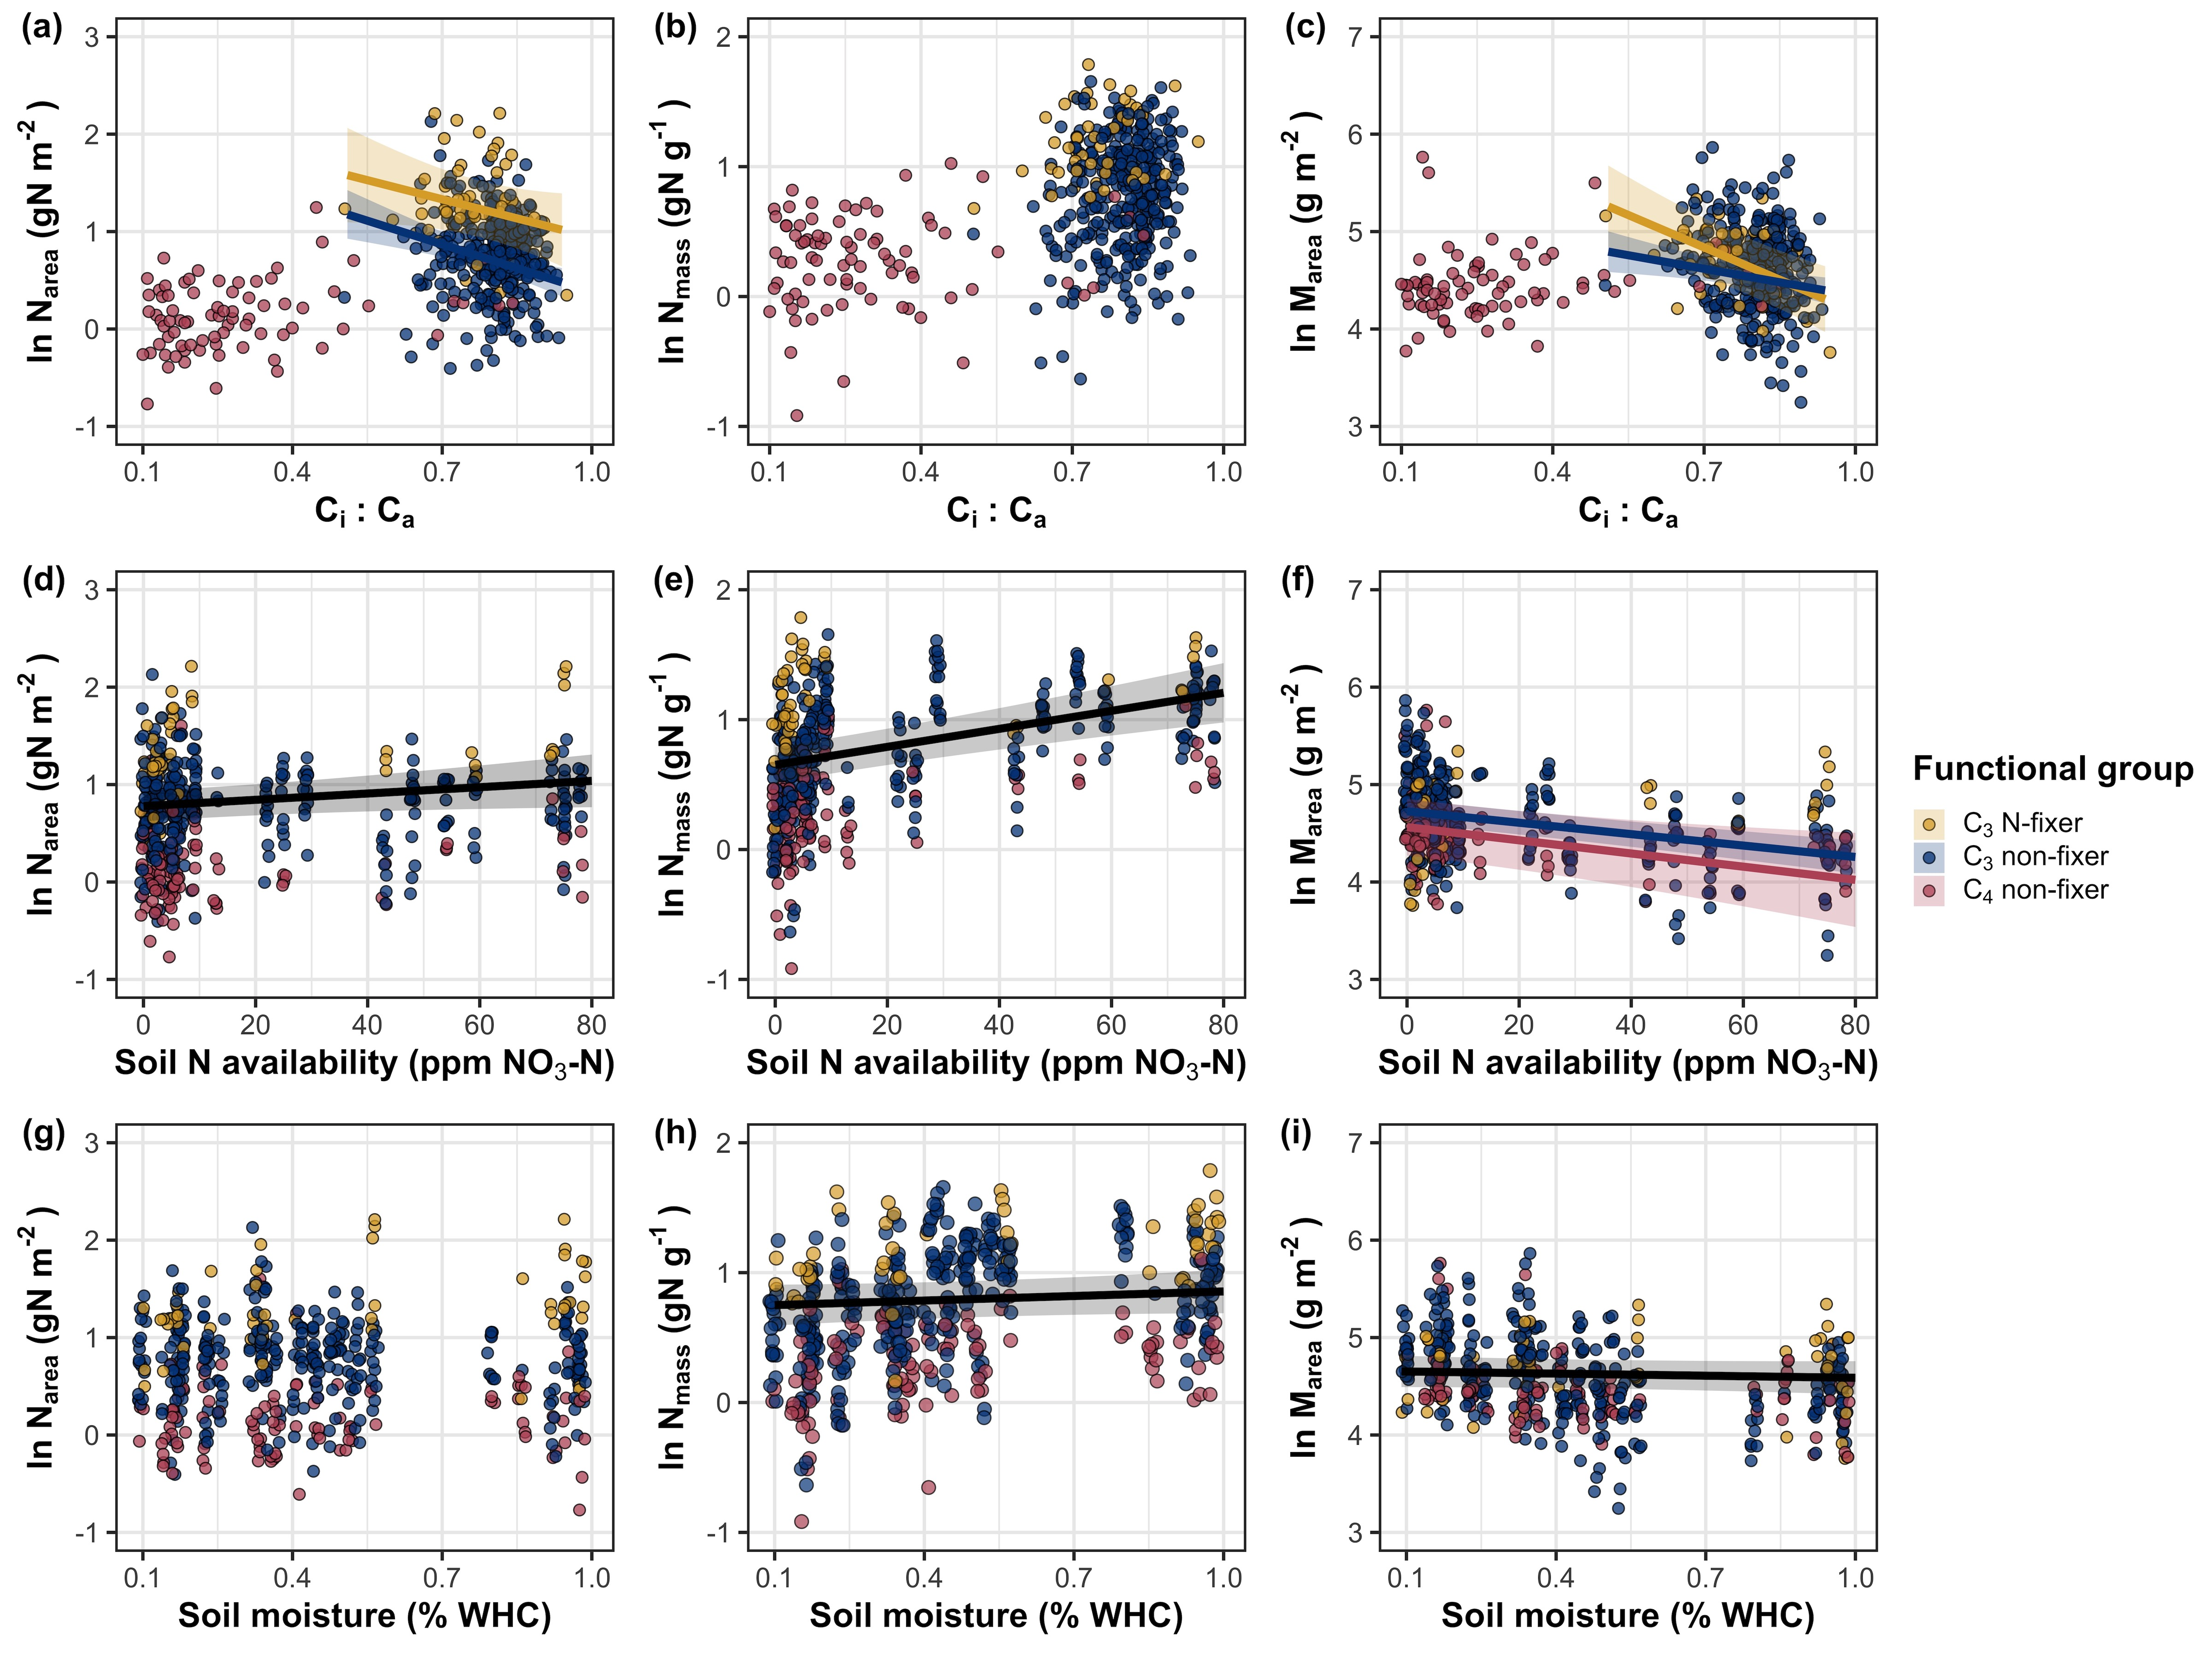
\includegraphics[scale = 0.045]{ch4_TXeco/figs/TXeco_fig4_narea.png}
        \caption[Effects of $\chi$, soil nitrogen availability, and soil moisture on leaf nitrogen content per unit leaf area, leaf nitrogen content per unit leaf biomass, and leaf mass per area.]{Effects of $\chi$ (a-c), soil nitrogen availability (d-f), and soil moisture (g-i) on leaf nitrogen content per unit leaf area (a, d, g), leaf nitrogen content per unit leaf biomass (b, e, h), and leaf mass per area (c, f, i). A solid black trendline indicates the bivariate relationship between the fixed effect the x-axis and response variable on the y-axis and is only included when there is no interaction between the x-axis and plant functional group.}
        \label{fig:figure4.4}
    \end{figure}
%\end{landscape}
\clearpage

\subsection{\textit{Structural equation model}}
The piecewise structural equation model explained 90\%, 54\%, 80\%, 92\%, and 41\% of variance in $N_\mathrm{area}$, $N_\mathrm{mass}$, $M_\mathrm{area}$, $\chi$, and $\beta$, respectively (Table 5; Fig. 5). Variance in $N_\mathrm{area}$ was driven by a negative effect of increasing $\chi$ (\textit{p} < 0.001; Table 5) paired with positive effects of increasing $N_\mathrm{mass}$ and $M_\mathrm{area}$ (\textit{p} < 0.001 in both cases; Table 5; Fig. 5). Model results indicated that the negative effect of $\chi$ on $N_\mathrm{area}$ was driven by a strong reduction in $M_\mathrm{area}$ with increasing $\chi$ (\textit{p} < 0.001; Table 5) paired with no change in $\chi$ due to Nmass (\textit{p} = 0.150; Table 5). However, there was a strong negative effect of increasing $M_\mathrm{area}$ on $N_\mathrm{mass}$ (\textit{p} < 0.001; Table 5; Fig. 5). $\chi$ generally increased with increasing $\beta$  (\textit{p} < 0.001; Table 5) and decreased with increasing VPD (\textit{p} < 0.001; Table 5; Fig. 5). Variance in $\beta$  was driven by a negative effect of increasing soil nitrogen availability (\textit{p} < 0.001; Table 5) and was generally higher in C$_3$ species (\textit{p} < 0.001; Table 5; Fig. 5). However, $\beta$ did not change with soil moisture (\textit{p} = 0.332; Table 5) or with ability to acquire nitrogen via symbiotic nitrogen fixation (\textit{p} = 0.546; Table 5). Finally, soil nitrogen availability was positively associated with increasing soil moisture (\textit{p} < 0.001; Table 5; Fig. 5), while VPD was negatively associated with increasing soil moisture (\textit{p} < 0.001; Table 5; Fig. 5).

\newpage
placeholder Table 5
\clearpage

\newpage
\begin{landscape}
    \begin{figure}
        \centering
        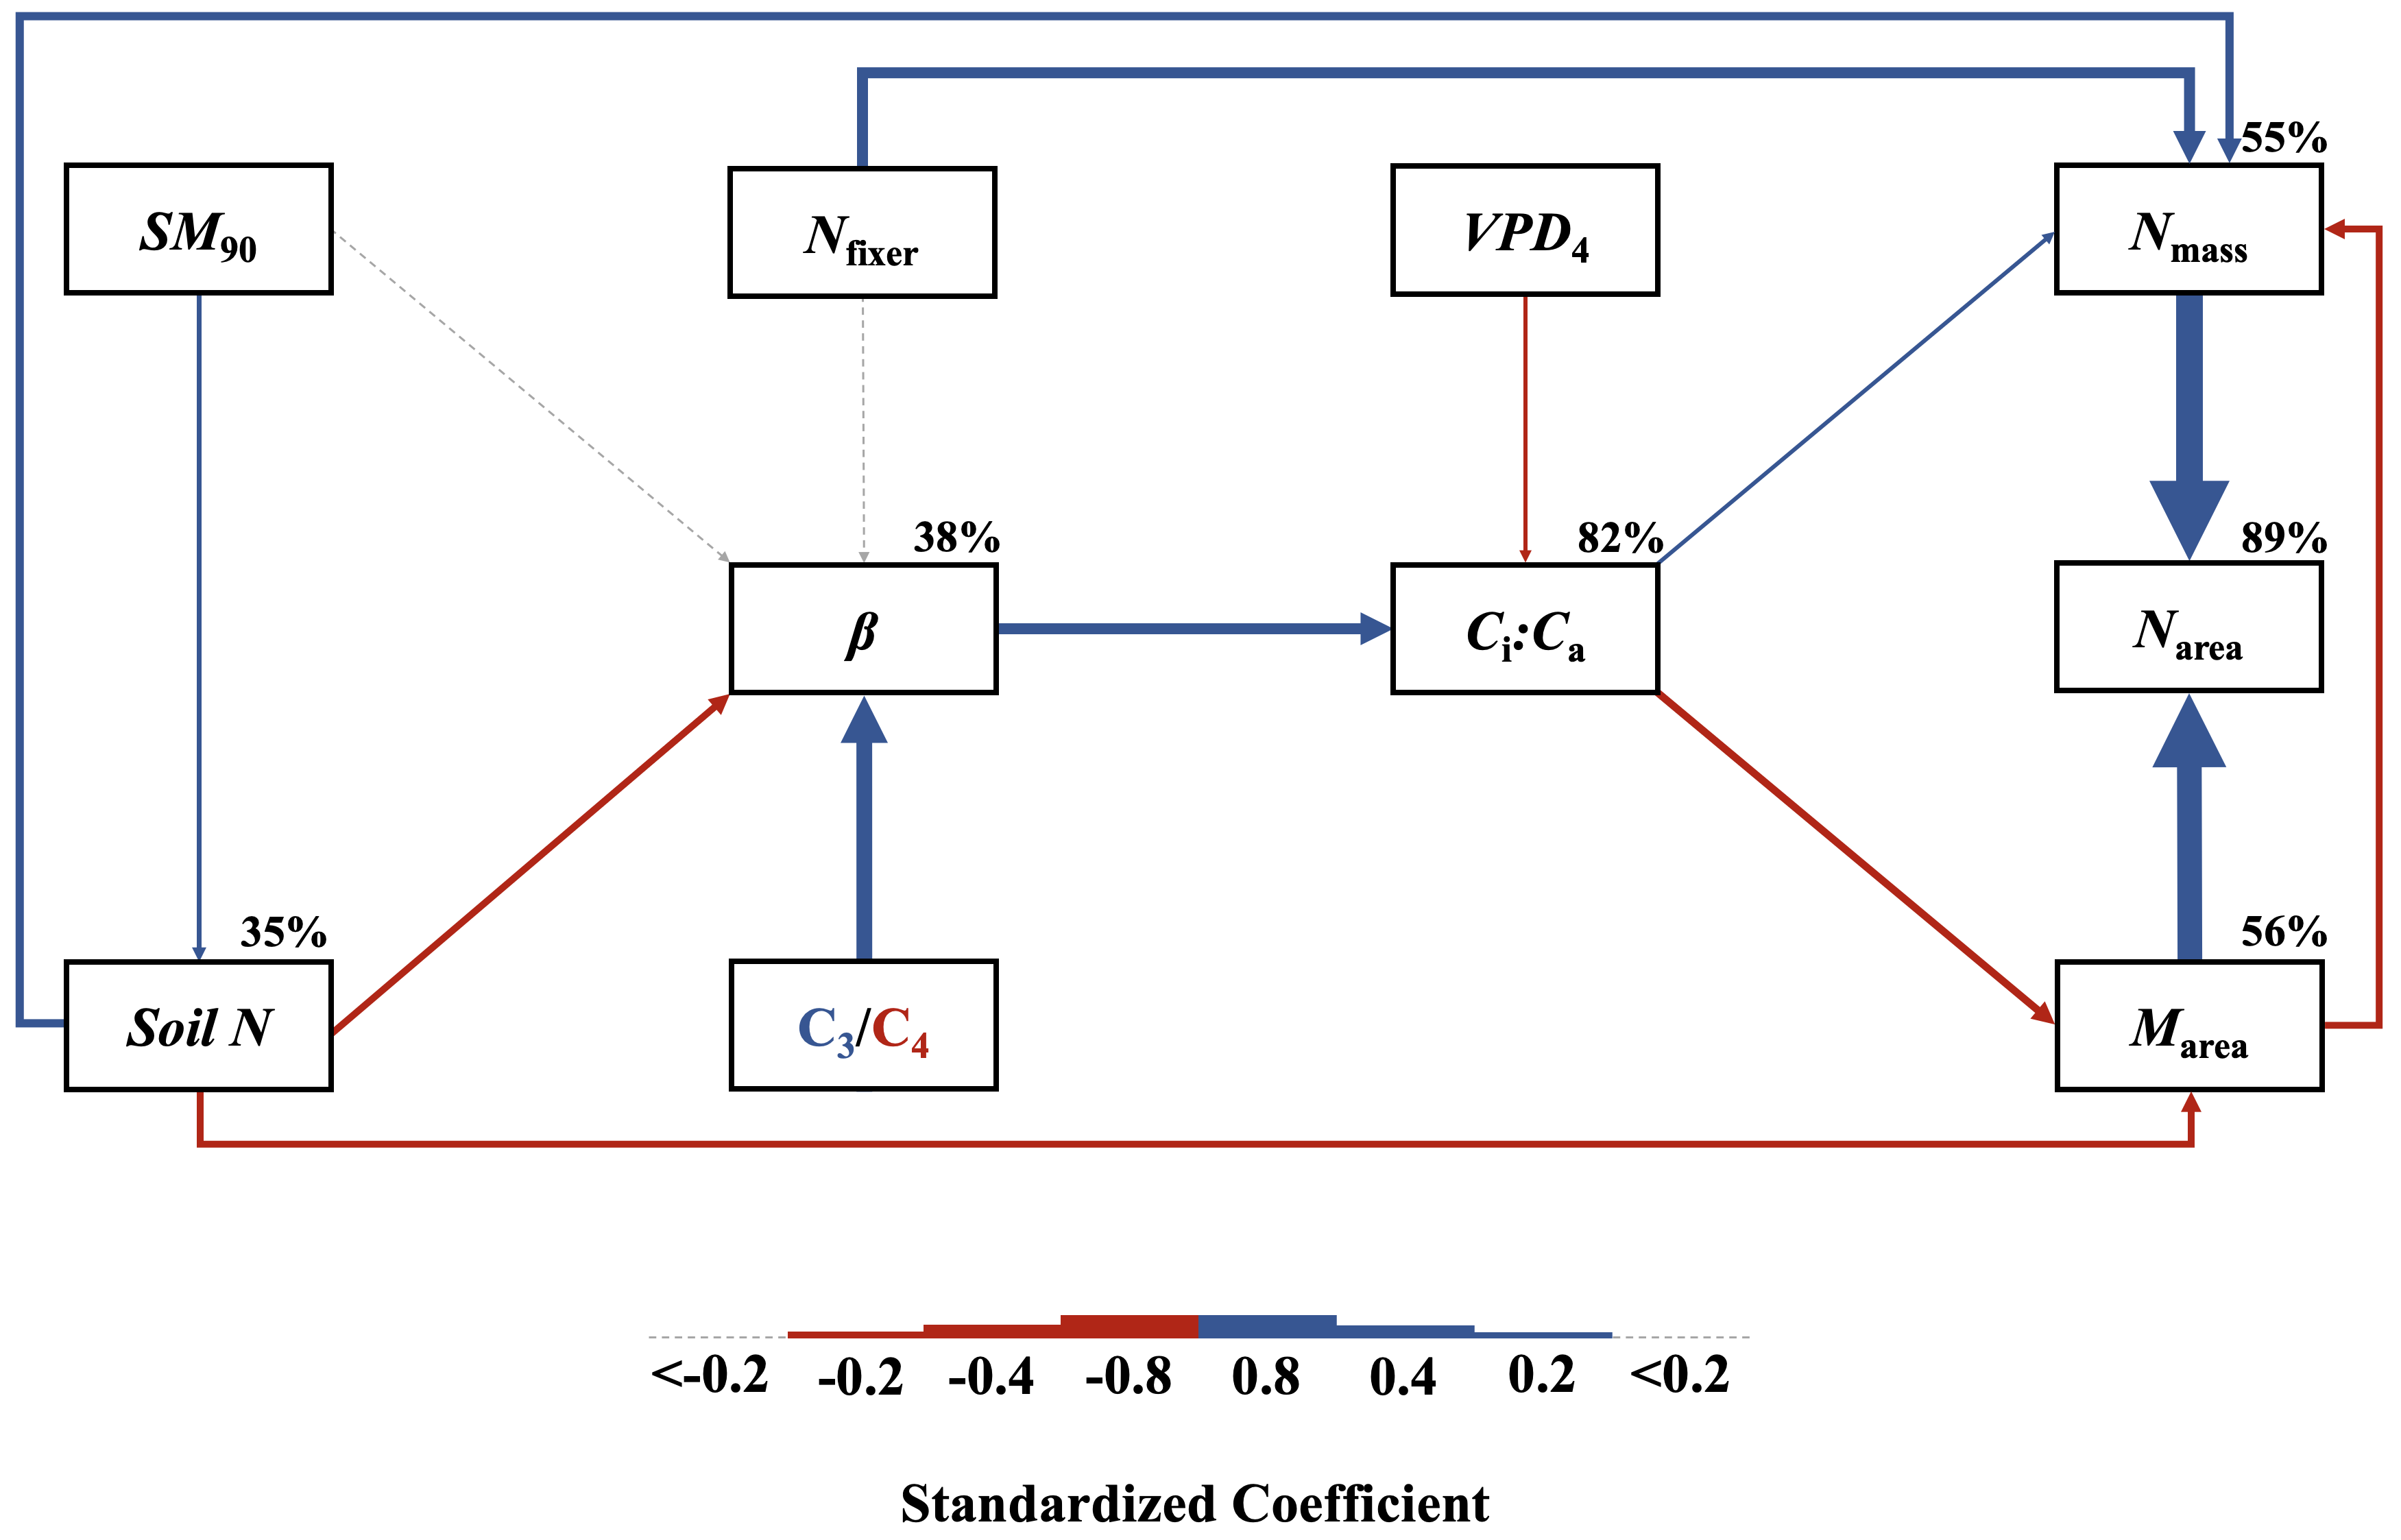
\includegraphics[scale = 0.3]{ch4_TXeco/figs/TXeco_fig5_SEM.png}
        \caption[Structural equation model results exploring direct and indirect drivers of $N_\mathrm{area}$]{Structural equation model results exploring direct and indirect drivers of $N_\mathrm{area}$. Boxes indicate measured edaphic factors, climatic factors, and leaf traits. Percentages above boxes indicate conditional $R^{2}$ values of each respective leaf trait. Solid arrows indicate bivariate relationships where \textit{p} < 0.05, while dashed arrows indicate bivariate relationships where \textit{p} > 0.05. Positive model coefficients are indicated through blue arrows, while negative model coefficients are indicated through red arrows. Arrow thickness scales with the standardized model coefficient of each bivariate relationship. A positive coefficient for photosynthetic pathway indicates generally larger values in C$_3$ species, while a positive coefficient for $N_\mathrm{fixer}$ indicates generally larger values in N-fixing species. Standardized model coefficients and associated \textit{p}-values are reported in Table 5.}
        \label{fig:figure4.5}
    \end{figure}
\end{landscape}
\clearpage


\section{Discussion}